
%% bare_conf.tex
%% V1.3
%% 2007/01/11
%% by Michael Shell
%% See:
%% http://www.michaelshell.org/
%% for current contact information.
%%
%% This is a skeleton file demonstrating the use of IEEEtran.cls
%% (requires IEEEtran.cls version 1.7 or later) with an IEEE conference paper.
%%
%% Support sites:
%% http://www.michaelshell.org/tex/ieeetran/
%% http://www.ctan.org/tex-archive/macros/latex/contrib/IEEEtran/
%% and
%% http://www.ieee.org/

%%*************************************************************************
%% Legal Notice:
%% This code is offered as-is without any warranty either expressed or
%% implied; without even the implied warranty of MERCHANTABILITY or
%% FITNESS FOR A PARTICULAR PURPOSE! 
%% User assumes all risk.
%% In no event shall IEEE or any contributor to this code be liable for
%% any damages or losses, including, but not limited to, incidental,
%% consequential, or any other damages, resulting from the use or misuse
%% of any information contained here.
%%
%% All comments are the opinions of their respective authors and are not
%% necessarily endorsed by the IEEE.
%%
%% This work is distributed under the LaTeX Project Public License (LPPL)
%% ( http://www.latex-project.org/ ) version 1.3, and may be freely used,
%% distributed and modified. A copy of the LPPL, version 1.3, is included
%% in the base LaTeX documentation of all distributions of LaTeX released
%% 2003/12/01 or later.
%% Retain all contribution notices and credits.
%% ** Modified files should be clearly indicated as such, including  **
%% ** renaming them and changing author support contact information. **
%%
%% File list of work: IEEEtran.cls, IEEEtran_HOWTO.pdf, bare_adv.tex,
%%                    bare_conf.tex, bare_jrnl.tex, bare_jrnl_compsoc.tex
%%*************************************************************************

% *** Authors should verify (and, if needed, correct) their LaTeX system  ***
% *** with the testflow diagnostic prior to trusting their LaTeX platform ***
% *** with production work. IEEE's font choices can trigger bugs that do  ***
% *** not appear when using other class files.                            ***
% The testflow support page is at:
% http://www.michaelshell.org/tex/testflow/



% Note that the a4paper option is mainly intended so that authors in
% countries using A4 can easily print to A4 and see how their papers will
% look in print - the typesetting of the document will not typically be
% affected with changes in paper size (but the bottom and side margins will).
% Use the testflow package mentioned above to verify correct handling of
% both paper sizes by the user's LaTeX system.
%
% Also note that the "draftcls" or "draftclsnofoot", not "draft", option
% should be used if it is desired that the figures are to be displayed in
% draft mode.
%
\documentclass[conference]{IEEEtran}
% Add the compsoc option for Computer Society conferences.
%
% If IEEEtran.cls has not been installed into the LaTeX system files,
% manually specify the path to it like:
% \documentclass[conference]{../sty/IEEEtran}
\usepackage{multirow}
\usepackage[table,xcdraw]{xcolor}

\usepackage{graphicx}
\usepackage{hyperref}
\usepackage{listings}
\usepackage{setspace}
\usepackage{caption}
\captionsetup[lstlisting]{position=bottom}

% Some very useful LaTeX packages include:
% (uncomment the ones you want to load)


% *** MISC UTILITY PACKAGES ***
%
%\usepackage{ifpdf}
% Heiko Oberdiek's ifpdf.sty is very useful if you need conditional
% compilation based on whether the output is pdf or dvi.
% usage:
% \ifpdf
%   % pdf code
% \else
%   % dvi code
% \fi
% The latest version of ifpdf.sty can be obtained from:
% http://www.ctan.org/tex-archive/macros/latex/contrib/oberdiek/
% Also, note that IEEEtran.cls V1.7 and later provides a builtin
% \ifCLASSINFOpdf conditional that works the same way.
% When switching from latex to pdflatex and vice-versa, the compiler may
% have to be run twice to clear warning/error messages.






% *** CITATION PACKAGES ***
%
%\usepackage{cite}
% cite.sty was written by Donald Arseneau
% V1.6 and later of IEEEtran pre-defines the format of the cite.sty package
% \cite{} output to follow that of IEEE. Loading the cite package will
% result in citation numbers being automatically sorted and properly
% "compressed/ranged". e.g., [1], [9], [2], [7], [5], [6] without using
% cite.sty will become [1], [2], [5]--[7], [9] using cite.sty. cite.sty's
% \cite will automatically add leading space, if needed. Use cite.sty's
% noadjust option (cite.sty V3.8 and later) if you want to turn this off.
% cite.sty is already installed on most LaTeX systems. Be sure and use
% version 4.0 (2003-05-27) and later if using hyperref.sty. cite.sty does
% not currently provide for hyperlinked citations.
% The latest version can be obtained at:
% http://www.ctan.org/tex-archive/macros/latex/contrib/cite/
% The documentation is contained in the cite.sty file itself.






% *** GRAPHICS RELATED PACKAGES ***
%
\ifCLASSINFOpdf
  % \usepackage[pdftex]{graphicx}
  % declare the path(s) where your graphic files are
  % \graphicspath{{../pdf/}{../jpeg/}}
  % and their extensions so you won't have to specify these with
  % every instance of \includegraphics
  % \DeclareGraphicsExtensions{.pdf,.jpeg,.png}
\else
  % or other class option (dvipsone, dvipdf, if not using dvips). graphicx
  % will default to the driver specified in the system graphics.cfg if no
  % driver is specified.
  % \usepackage[dvips]{graphicx}
  % declare the path(s) where your graphic files are
  % \graphicspath{{../eps/}}
  % and their extensions so you won't have to specify these with
  % every instance of \includegraphics
  % \DeclareGraphicsExtensions{.eps}
\fi
% graphicx was written by David Carlisle and Sebastian Rahtz. It is
% required if you want graphics, photos, etc. graphicx.sty is already
% installed on most LaTeX systems. The latest version and documentation can
% be obtained at: 
% http://www.ctan.org/tex-archive/macros/latex/required/graphics/
% Another good source of documentation is "Using Imported Graphics in
% LaTeX2e" by Keith Reckdahl which can be found as epslatex.ps or
% epslatex.pdf at: http://www.ctan.org/tex-archive/info/
%
% latex, and pdflatex in dvi mode, support graphics in encapsulated
% postscript (.eps) format. pdflatex in pdf mode supports graphics
% in .pdf, .jpeg, .png and .mps (metapost) formats. Users should ensure
% that all non-photo figures use a vector format (.eps, .pdf, .mps) and
% not a bitmapped formats (.jpeg, .png). IEEE frowns on bitmapped formats
% which can result in "jaggedy"/blurry rendering of lines and letters as
% well as large increases in file sizes.
%
% You can find documentation about the pdfTeX application at:
% http://www.tug.org/applications/pdftex





% *** MATH PACKAGES ***
%
%\usepackage[cmex10]{amsmath}
% A popular package from the American Mathematical Society that provides
% many useful and powerful commands for dealing with mathematics. If using
% it, be sure to load this package with the cmex10 option to ensure that
% only type 1 fonts will utilized at all point sizes. Without this option,
% it is possible that some math symbols, particularly those within
% footnotes, will be rendered in bitmap form which will result in a
% document that can not be IEEE Xplore compliant!
%
% Also, note that the amsmath package sets \interdisplaylinepenalty to 10000
% thus preventing page breaks from occurring within multiline equations. Use:
%\interdisplaylinepenalty=2500
% after loading amsmath to restore such page breaks as IEEEtran.cls normally
% does. amsmath.sty is already installed on most LaTeX systems. The latest
% version and documentation can be obtained at:
% http://www.ctan.org/tex-archive/macros/latex/required/amslatex/math/





% *** SPECIALIZED LIST PACKAGES ***
%
\usepackage[activate={true,nocompatibility},final,tracking=true,kerning=true,spacing=true,factor=1100,stretch=10,shrink=10]{microtype}
\usepackage{algorithm}
\usepackage{algpseudocode}
\usepackage{algorithmicx}
\algnewcommand\algorithmicinput{\textbf{INPUT:}}
\algnewcommand\INPUT{\item[\algorithmicinput]}
\algnewcommand\algorithmicoutput{\textbf{OUTPUT:}}
\algnewcommand\OUTPUT{\item[\algorithmicoutput]}
\algnotext{EndFor}
\algnotext{EndIf}
\algnotext{EndWhile}
% algorithmic.sty was written by Peter Williams and Rogerio Brito.
% This package provides an algorithmic environment fo describing algorithms.
% You can use the algorithmic environment in-text or within a figure
% environment to provide for a floating algorithm. Do NOT use the algorithm
% floating environment provided by algorithm.sty (by the same authors) or
% algorithm2e.sty (by Christophe Fiorio) as IEEE does not use dedicated
% algorithm float types and packages that provide these will not provide
% correct IEEE style captions. The latest version and documentation of
% algorithmic.sty can be obtained at:
% http://www.ctan.org/tex-archive/macros/latex/contrib/algorithms/
% There is also a support site at:
% http://algorithms.berlios.de/index.html
% Also of interest may be the (relatively newer and more customizable)
% algorithmicx.sty package by Szasz Janos:
% http://www.ctan.org/tex-archive/macros/latex/contrib/algorithmicx/



% *** ALIGNMENT PACKAGES ***
%
%\usepackage{array}
% Frank Mittelbach's and David Carlisle's array.sty patches and improves
% the standard LaTeX2e array and tabular environments to provide better
% appearance and additional user controls. As the default LaTeX2e table
% generation code is lacking to the point of almost being broken with
% respect to the quality of the end results, all users are strongly
% advised to use an enhanced (at the very least that provided by array.sty)
% set of table tools. array.sty is already installed on most systems. The
% latest version and documentation can be obtained at:
% http://www.ctan.org/tex-archive/macros/latex/required/tools/


%\usepackage{mdwmath}
%\usepackage{mdwtab}
% Also highly recommended is Mark Wooding's extremely powerful MDW tools,
% especially mdwmath.sty and mdwtab.sty which are used to format equations
% and tables, respectively. The MDWtools set is already installed on most
% LaTeX systems. The lastest version and documentation is available at:
% http://www.ctan.org/tex-archive/macros/latex/contrib/mdwtools/


% IEEEtran contains the IEEEeqnarray family of commands that can be used to
% generate multiline equations as well as matrices, tables, etc., of high
% quality.


%\usepackage{eqparbox}
% Also of notable interest is Scott Pakin's eqparbox package for creating
% (automatically sized) equal width boxes - aka "natural width parboxes".
% Available at:
% http://www.ctan.org/tex-archive/macros/latex/contrib/eqparbox/





% *** SUBFIGURE PACKAGES ***
%\usepackage[tight,footnotesize]{subfigure}
% subfigure.sty was written by Steven Douglas Cochran. This package makes it
% easy to put subfigures in your figures. e.g., "Figure 1a and 1b". For IEEE
% work, it is a good idea to load it with the tight package option to reduce
% the amount of white space around the subfigures. subfigure.sty is already
% installed on most LaTeX systems. The latest version and documentation can
% be obtained at:
% http://www.ctan.org/tex-archive/obsolete/macros/latex/contrib/subfigure/
% subfigure.sty has been superceeded by subfig.sty.



%\usepackage[caption=false]{caption}
%\usepackage[font=footnotesize]{subfig}
% subfig.sty, also written by Steven Douglas Cochran, is the modern
% replacement for subfigure.sty. However, subfig.sty requires and
% automatically loads Axel Sommerfeldt's caption.sty which will override
% IEEEtran.cls handling of captions and this will result in nonIEEE style
% figure/table captions. To prevent this problem, be sure and preload
% caption.sty with its "caption=false" package option. This is will preserve
% IEEEtran.cls handing of captions. Version 1.3 (2005/06/28) and later 
% (recommended due to many improvements over 1.2) of subfig.sty supports
% the caption=false option directly:
%\usepackage[caption=false,font=footnotesize]{subfig}
%
% The latest version and documentation can be obtained at:
% http://www.ctan.org/tex-archive/macros/latex/contrib/subfig/
% The latest version and documentation of caption.sty can be obtained at:
% http://www.ctan.org/tex-archive/macros/latex/contrib/caption/




% *** FLOAT PACKAGES ***
%
%\usepackage{fixltx2e}
% fixltx2e, the successor to the earlier fix2col.sty, was written by
% Frank Mittelbach and David Carlisle. This package corrects a few problems
% in the LaTeX2e kernel, the most notable of which is that in current
% LaTeX2e releases, the ordering of single and double column floats is not
% guaranteed to be preserved. Thus, an unpatched LaTeX2e can allow a
% single column figure to be placed prior to an earlier double column
% figure. The latest version and documentation can be found at:
% http://www.ctan.org/tex-archive/macros/latex/base/



%\usepackage{stfloats}
% stfloats.sty was written by Sigitas Tolusis. This package gives LaTeX2e
% the ability to do double column floats at the bottom of the page as well
% as the top. (e.g., "\begin{figure*}[!b]" is not normally possible in
% LaTeX2e). It also provides a command:
%\fnbelowfloat
% to enable the placement of footnotes below bottom floats (the standard
% LaTeX2e kernel puts them above bottom floats). This is an invasive package
% which rewrites many portions of the LaTeX2e float routines. It may not work
% with other packages that modify the LaTeX2e float routines. The latest
% version and documentation can be obtained at:
% http://www.ctan.org/tex-archive/macros/latex/contrib/sttools/
% Documentation is contained in the stfloats.sty comments as well as in the
% presfull.pdf file. Do not use the stfloats baselinefloat ability as IEEE
% does not allow \baselineskip to stretch. Authors submitting work to the
% IEEE should note that IEEE rarely uses double column equations and
% that authors should try to avoid such use. Do not be tempted to use the
% cuted.sty or midfloat.sty packages (also by Sigitas Tolusis) as IEEE does
% not format its papers in such ways.





% *** PDF, URL AND HYPERLINK PACKAGES ***
%
%\usepackage{url}
% url.sty was written by Donald Arseneau. It provides better support for
% handling and breaking URLs. url.sty is already installed on most LaTeX
% systems. The latest version can be obtained at:
% http://www.ctan.org/tex-archive/macros/latex/contrib/misc/
% Read the url.sty source comments for usage information. Basically,
% \url{my_url_here}.





% *** Do not adjust lengths that control margins, column widths, etc. ***
% *** Do not use packages that alter fonts (such as pslatex).         ***
% There should be no need to do such things with IEEEtran.cls V1.6 and later.
% (Unless specifically asked to do so by the journal or conference you plan
% to submit to, of course. )


% correct bad hyphenation here
\hyphenation{op-tical net-works semi-conduc-tor}


\begin{document}
%
% paper title
% can use linebreaks \\ within to get better formatting as desired
\title{StitchUp: Automatic Control Flow Protection for High Level Synthesis Tools\vspace{-10mm}}


% author names and affiliations
% use a multiple column layout for up to three different
% affiliations
\author{\IEEEauthorblockN{Shane T. Fleming and David B. Thomas}
\IEEEauthorblockA{Dept Electrical and Electronic Engineering, Imperial College London, email: \{sf306, d.thomas1\}@ic.ac.uk}
}
% conference papers do not typically use \thanks and this command
% is locked out in conference mode. If really needed, such as for
% the acknowledgment of grants, issue a \IEEEoverridecommandlockouts
% after \documentclass

% for over three affiliations, or if they all won't fit within the width
% of the page, use this alternative format:
% 
%\author{\IEEEauthorblockN{Michael Shell\IEEEauthorrefmark{1},
%Homer Simpson\IEEEauthorrefmark{2},
%James Kirk\IEEEauthorrefmark{3}, 
%Montgomery Scott\IEEEauthorrefmark{3} and
%Eldon Tyrell\IEEEauthorrefmark{4}}
%\IEEEauthorblockA{\IEEEauthorrefmark{1}School of Electrical and Computer Engineering\\
%Georgia Institute of Technology,
%Atlanta, Georgia 30332--0250\\ Email: see http://www.michaelshell.org/contact.html}
%\IEEEauthorblockA{\IEEEauthorrefmark{2}Twentieth Century Fox, Springfield, USA\\
%Email: homer@thesimpsons.com}
%\IEEEauthorblockA{\IEEEauthorrefmark{3}Starfleet Academy, San Francisco, California 96678-2391\\
%Telephone: (800) 555--1212, Fax: (888) 555--1212}
%\IEEEauthorblockA{\IEEEauthorrefmark{4}Tyrell Inc., 123 Replicant Street, Los Angeles, California 90210--4321}}




% use for special paper notices
%\IEEEspecialpapernotice{(Invited Paper)}




% make the title area
\maketitle


\begin{abstract}
%\boldmath
Soft-error detection in FPGAs typically requires replication,
doubling the required area.
We propose an approach which distinguishes
between tolerable errors in data-flow, such-as arithmetic,
and intolerable errors in control-flow, such as branches and their data-dependencies.
This approach is demonstrated in a new high-level synthesis
compiler pass
called StitchUp, which precisely identifies the control critical
parts of the design, then automatically replicates only that part.
We applied StitchUp to the CHStone benchmark suite and performed
exhaustive error injection in hardware, finding that 99.99\% of all control-flow errors were detected, and a best-case 95\% reduction
in area overhead versus naive replication.
\end{abstract}
% IEEEtran.cls defaults to using nonbold math in the Abstract.
% This preserves the distinction between vectors and scalars. However,
% if the conference you are submitting to favors bold math in the abstract,
% then you can use LaTeX's standard command \boldmath at the very start
% of the abstract to achieve this. Many IEEE journals/conferences frown on
% math in the abstract anyway.

% no keywords




% For peer review papers, you can put extra information on the cover
% page as needed:
% \ifCLASSOPTIONpeerreview
% \begin{center} \bfseries EDICS Category: 3-BBND \end{center}
% \fi
%
% For peerreview papers, this IEEEtran command inserts a page break and
% creates the second title. It will be ignored for other modes.
\IEEEpeerreviewmaketitle



\section{Introduction}
\providecommand*{\lstnumberautorefname}{line}

High-level Synthesis tools, like LegUp or VivadoHLS, can automatically generate an FPGA 
circuit for the matrix multiplication example in Listing \ref{lst:MMM}.
What if the designer was required to run this circuit reliably in the
presence of soft errors? 
The naive approach would be to instantiate multiple copies of the circuit and run
them in lock-step on the same input data with any deviations between them
indicating an error.

 \lstset{
         basicstyle=\footnotesize\ttfamily, % Standardschrift
         numbers=left,               % Ort der Zeilennummern
         numberstyle=\tiny,          % Stil der Zeilennummern
	 language=C,
         %stepnumber=2,               % Abstand zwischen den Zeilennummern
         numbersep=5pt,              % Abstand der Nummern zum Text
         tabsize=2,                  % Groesse von Tabs
         extendedchars=true,         %
         breaklines=true,            % Zeilen werden Umgebrochen
         keywordstyle=\color{red},
         %frame=b,         
 %        keywordstyle=[1]\textbf,    % Stil der Keywords
 %        keywordstyle=[2]\textbf,    %
 %        keywordstyle=[3]\textbf,    %
 %        keywordstyle=[4]\textbf,   \sqrt{\sqrt{}} %
         stringstyle=\color{white}\ttfamily, % Farbe der String
         showspaces=false,           % Leerzeichen anzeigen ?
         showtabs=false,             % Tabs anzeigen ?
         %xleftmargin=10pt,
         %framexleftmargin=17pt,
         %framexrightmargin=5pt,
         %framexbottommargin=4pt,
         %backgroundcolor=\color{lightgray},
         showstringspaces=false      % Leerzeichen in Strings anzeigen ?        
 }


Replication in this fashion is expensive in both area and more importantly
power, especially in this example as expensive floating point arithmetic
units are required for the calculation of the inner dot product.

If tight constraints prevent full replication then reliability can still be
improved through selectively replicating "important" portions of the design.
Various studies have shown that for a number of applications there exist critical regions
of code sensitive to soft errors and non-critical regions which are less sensitive.
This is especially true in applications involving media processing or machine
learning\cite{wong2006soft} \cite{liu2012flikker}.

%What about just the control flow?
Control-flow regions, (i.e. instructions effecting branch decisions), are arguably more critical
than data-flow, since faults within control-flow can effect real time guarantees
and termination.
Research into HLS for VLSI designs has proved promising for control-flow intensive
(CFI) applications \cite{chen2014reliability,chen2015reliability}, and fault injection
results have shown that control-flows are highly vulnerable to errors
\cite{saggese2005microprocessor, nakka2007processor, wong2006soft}.

%In our example what would control flow errors do?
Faults within the control structure for our matrix multiplication example
could cause the calculation of rows and columns of the output matrix \lstinline$C$ to be skipped,
or even worse, cause the circuit to enter an infinite loop and never terminate.
This paper presents an approach for automatically extracting the control flow structure
for a HLS application so that this region of the design can be selectively
replicated to protect control decisions.

%\begin{figure}[t]
%\centering
%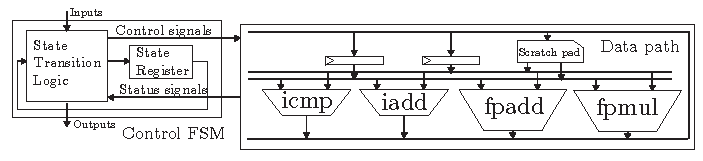
\includegraphics[width=3.5in]{./imgs/singleHLSArch_v2.pdf}
%\caption{Diagram representing a HLS circuit for the Matrix Multiplication example}
%\label{fig:singleHLSArch}
%\end{figure}


\begin{figure}[t]
\begin{lstlisting}[label={lst:MMM}, captionpos=b, caption={Matrix Multiplication Example}]
void MMM(float A[5][5],float B[5][5],float C[5][5])
{ int i=0, j=0, k=0;
  for(i=0, i<5, i++){
    for(j=0, j<5; j++){
      C[i][j] = 0;
      for(k=0, k<5; k++){
        C[i][j] += A[i][k]*B[k][j]; }
    }
  }
}
\end{lstlisting}
\vspace{-7mm}
\end{figure}

Figure \ref{fig:singleHLSArch} provides a diagram of the HLS generated
circuit for our matrix multiplication example.
Two clear partitions can be seen, a data path where functional units reside, and a
control FSM responsible for scheduling instructions onto the functional units.
In order to replicate only the control-flow structure
any data-path functional units which may influence a state transition need to be
duplicated along with the control FSM.

Analysing the code in Listing \ref{lst:MMM} we can determine that the instructions
which influence control-flow decisions are the ones used in the \lstinline{for} loop
conditions, which require an integer comparator \textbf{icmp} and adder \textbf{iadd}.
While the expensive floating point units, \textbf{fpmul} and \textbf{fpadd}, required
for calculating the inner dot product on line 7 have no
influence over any branch decision and will not be replicated.

Manually inspecting code and removing elements that don't influence control flow
may be feasible in the simple case of Matrix Multiplication, however as the complexity of the input increases
the engineering effort required in both analysing the input source and a generating circuit with an identical control FSM is
significant.
StitchUp fully automates this process through using a static analysis technique, known as program slicing, to extract
and duplicate any instructions that may influence control. The contribution of this paper are:

\vspace{-4pt}
\begin{itemize}
	\setlength{\itemsep}{1pt}
	\setlength{\parskip}{0pt}
	\setlength{\parsep}{0pt}
	\item StitchUp, a tool which can automatically extract and protect the control flow structure of a circuit generated with a HLS tool.
	\item Detailed results of StitchUp on the CHStone benchmark, where exhaustive hardware fault injection is performed on the majority of cases.
	\item Results exploring the reliability of StitchUp protected circuits as the control to data ratio is varied through
	loop unrolling in the matrix multiplication example.
\end{itemize}
%\vspace{1mm}
%\noindent
%$\bullet$ StitchUp, a tool which can automatically extract and protect the control flow structure of a circuit generated with a HLS tool.
%
%\vspace{1mm}
%\noindent
%$\bullet$ Detailed results of StitchUp on the CHStone benchmark, where exhaustive hardware fault injection is performed on the majority of cases.
%
%\vspace{1mm}
%\noindent
%$\bullet$ Results exploring the reliability of StitchUp protected circuits as the control to data ratio is varied through loop unrolling in the matrix multiplication example.


\section{FPGA device faults due to soft-errors}
\begin{figure}[t]
\centering
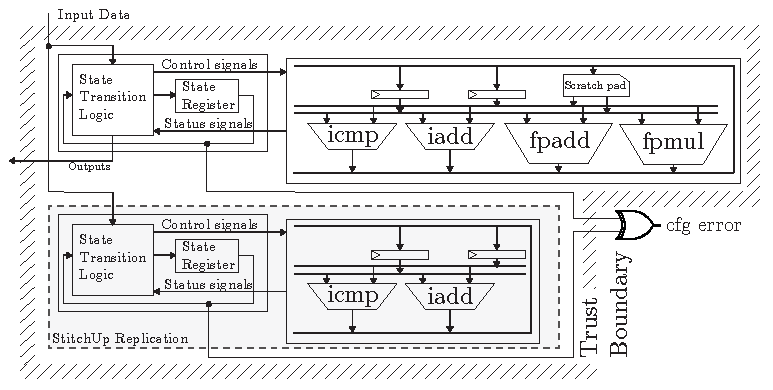
\includegraphics[width=3.5in]{./imgs/StitchUpReplication.pdf}
\caption{Default circuit (a) and Control Replicant (b) for our Dot Product example in Listing \ref{lst:DotProduct}, with Trust Boundary \vspace{-5mm}}
\label{fig:HLSArch}
\end{figure}

A Soft Error or Single Event Upset is a random, non-catastrophic error, where radiation causes
a perturbation to a circuit by temporarily altering a single signal or datum.
Detecting and mitigating such errors is important in some fields, such as satellite design,
where high design costs, \textbf{harsh environments}, and the difficulties in repairing once deployed make it necessary.
Additionally, due to the continuing increase in semiconductor density, the current soft error challenges 
experienced in space will also occur in future terrestrial devices.\cite{normand1996single}\cite{henkel2013reliable}.

FPGA devices work by mapping circuit descriptions into a collection of Logic Elements,
which are described in programmable Look-Up-Tables (LUTs) and routed together via
programmable switchboxes.
Configuration data for both the look-up-tables and switchboxes are stored in an SRAM based
configuration memory, which means soft errors can either change the functionality
of Logic Elements or can change the routing between them.
Other memories called block memory and flip-flops are also present in FPGA devices,
and soft errors in these regions can cause transient errors in the circuit.

%How this changes the protection strategy compared to software and VLSI
For ASIC designs, registers are the most vulnerable to soft-errors with
combinational logic contributing very little to overall circuit relability \cite{baumann2005soft}.
This makes ASIC approaches which analyses and protect vulnerable registers, such as in \cite{chen2014reliability},
promising approaches.
However in FPGA devices the most vulnerable region is the SRAM based configuration memory,
so such approaches would have little impact requiring methods perform combinatorial logic
replication such as StitchUp or DMR/TMR.

%ECC and frame based checking approaches
Circuits described within configuration memory are usually protected in one of two ways:
(1)the circuit is replicated with comparison; (2)ECC/CRC signals associated with
frames of the configuration memory are regularly scanned for errors.
Replication uses extra area and power but has low error detection latency and can
protect both configuration memory and registers,
while ECC/CRC checks consume less area and power in exchange for higher detection 
latency and an inability to protect registers.

For this paper our \emph{fault model} assumes that a single soft error
can occur at most every clock cycle, and that this error can effect block memory,
SRAM configuration memory, or flip-flops.
Since errors are not solely within the configuration memory, replication must be used,
as configuration ECC/CRC cannot protect the registers in our control structure.
Figure \ref{fig:HLSArch} shows a StitchUp generated circuit for the dot product 
example in Listing \ref{lst:DotProduct}, with the original circuit on top and the
control-flow structure shadow beneath it.
StitchUp aims to protect all configuration, block, and Flip-flop bits within the
trust boundary (grey box) as everything outside, such as routing to
external I/O or DDR, is not protected.



\section{StitchUp Overview} %Talk generally about the tool and what we are aiming to protect (Formal stuff goes here)

\subsection{Tool-Flow}


\begin{figure*}[t]
\centering
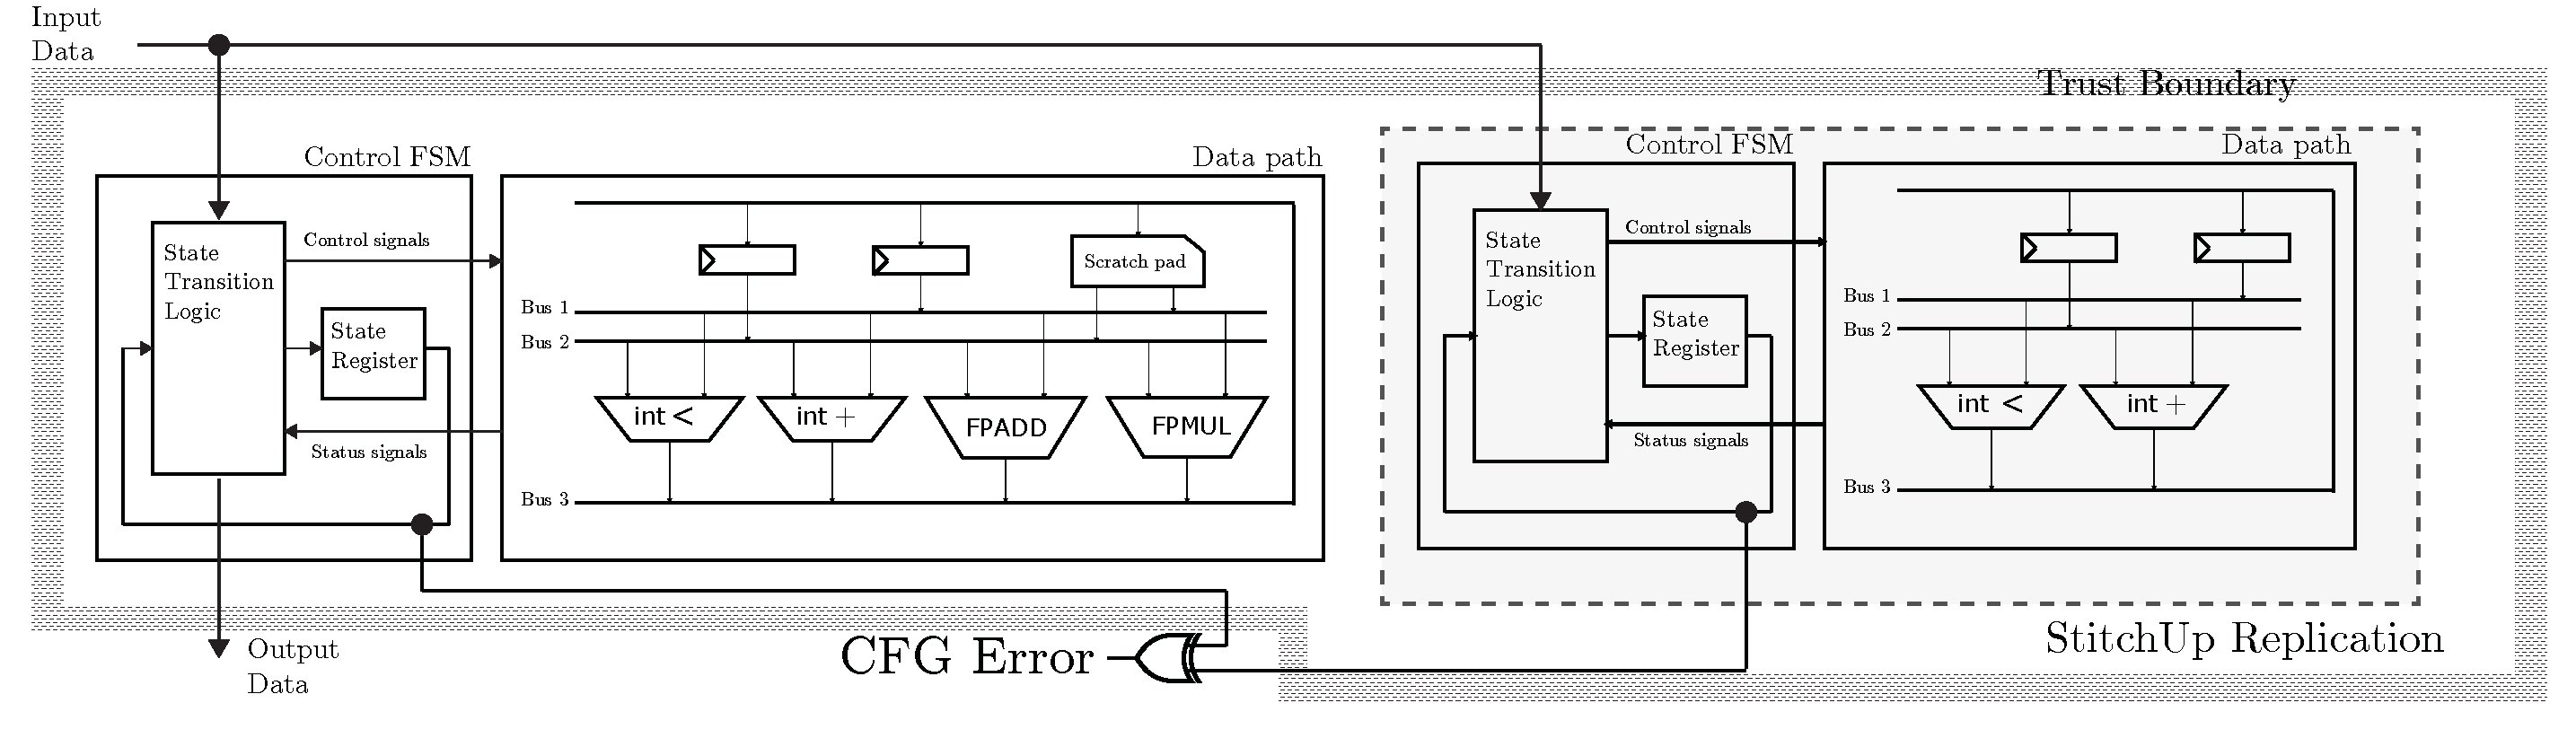
\includegraphics[width=7in]{./imgs/HLSArch.pdf}
\caption{StitchUp Replication for the Matrix Multiplication example, with Trust Boundary}
\label{fig:HLSArch}
\end{figure*}


\begin{figure}[h]
\centering
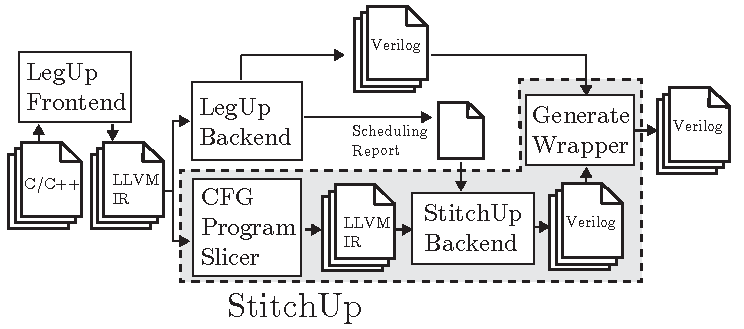
\includegraphics[width=3.5in]{./imgs/tool-flow.pdf}
\caption{Tool Flow Overview diagram}
\label{fig:tool_flow_diagram}
\end{figure}

StitchUp is built as a compile flag for LegUp an open source HLS tool built upon LLVM intermediate representation (LLVM-IR) which has
a similar level of abstraction to assembly code.
LLVM-IR has two important features for writing compiler optimisations:
firstly all instructions are in single static assignment form (SSA) where every variable is only
assigned once; and secondly instructions are grouped into straight-line sequences known as basic blocks (BB)
where there can only one branch in at the start of the block, and one branch out at the end.

Figure \ref{fig:tool_flow_diagram} shows the transformation of an input C program, to a Control-flow protected
Verilog output circuit, with StitchUp specific regions highlighted in grey.
Initially the C input is passed into the LegUp frontend, which is organised as a series of LLVM passes which
to perform various tasks such as annotating instructions with pipelining information.
The LegUp frontend outputs some LLVM-IR which is passed into both the backend of LegUp, to generate the full
original version of the circuit, and the frontend of StitchUp which will generate a control structure only version
of the original circuit.


\begin{figure}[h]
\centering
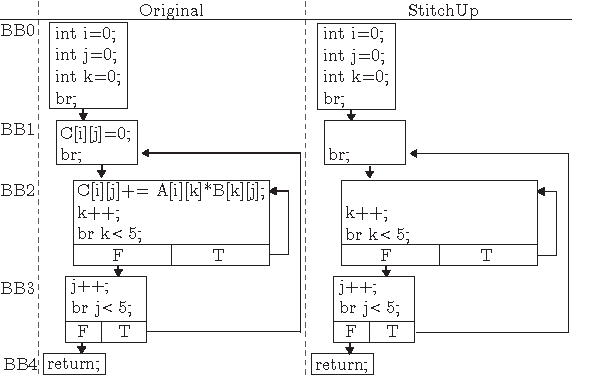
\includegraphics[width=3.5in]{./imgs/mmm_cdfg.pdf}
\caption{Control-Data-Flow Diagram for Matrix Multiplication example}
\label{fig:mmm_cdfg}
\end{figure}

\subsection{Extracting the Control Instruction Set}
The LLVM-IR which is passed into the frontend of StitchUp is naturally arranged into a Control and Dataflow graph (CDFG) format,
where each node of the graph is a basic block and edges are the branches between them.
An example of the CDFG for the matrix multiplication in listing \ref{lst:MMM} is shown on the left in Figure \ref{fig:mmm_cdfg}.

The aim of the StitchUp frontend is to extract all SSA instructions that influence any branch decision and collect them into what
we refer to as a Control Structure Instruction Set (CSIS), which can then be used to generate a control structure only circuit.
In Figure \ref{fig:mmm_cdfg} the original CDFG and StitchUp CDFG can be seen side by side, the CSIS for this example
is every instruction within the StitchUp CDFG and it can be seen that the floating point inner dot product calculation
is not there since it has no impact on any control decision.

In order to automatically extract the $CSIS$ a backwards analysis walks up from the final node of the CDFG to the starting node, analysing
the code as it goes and creating a $CSIS_{i}$ where $i$ is the current node.
The overall $CSIS$ for the input is $CSIS_s$ where $s$ is the starting node of the CDFG.
Constructing the $CSIS_i$ for each node $i$ requires the following three steps:
\begin{enumerate}
    \item For all successor nodes, $j$, of $i$ add every element of $CSIS_j$ to $CSIS_i$.
    \item All branch instructions and operands are added to $CSIS_i$
    \item Any instruction within $i$ that is used as an operand by an element of $CSIS_i$ is added to $CSIS_i$
\end{enumerate}

Following through the example in \ref{fig:mmm_cdfg}:
\begin{itemize}
\item initially start at $BB4$ attempting to build $CSIS_{BB4}$:
since $BB4$ has no successor nodes the first step is skipped, however for the second step the \lstinline{return}
instruction is added to $CSIS_{BB4}$, and the third step is skipped since no other instructions exist.

\item Moving backwards to $BB3$ the first step adds every element of $CSIS_{BB4}$ to $CSIS_{BB3}$ to give 
$CSIS_{BB3}=$ \{\lstinline{return}\}, then since $CSIS_{BB1}$ is currently empty nothing is added from here; the second step then adds the conditional branch and it's operand
instruction to the current set to give $CSIS_{BB3}= $\{\lstinline{return}, \lstinline{br j<5}\} ;
finally for step 3 \lstinline{j} is used in a member of $CSIS_{BB3}$ in \lstinline{br j<5} so the instruction
\lstinline{j++} is added to $CSIS_{BB3}$. This means that at this point $CSIS_{BB3} =$
\{\lstinline{return},\lstinline{br j<5}, \lstinline{j++}\}

\item For $BB2$ in the first step we take all the elements from the successor node $BB3$, and ignore the fact
that it has itself as a successor, so that we get $CSIS_{BB2} =$ \{\lstinline{return},\lstinline{br j<5}, \lstinline{j++}\}.
Then just like before we can add the branch instruction, \lstinline{br k<5}, using rule 2 and the incrementor for the branch
conditional variable \lstinline{k} using rule 3. 
The instruction \lstinline{C[i][j] += A[i][k]*B[k][j]} is not added to $CSIS_{BB2}$ since no instruction
within $CSIS_{BB2}$ depends on it. This leaves 

\end{itemize}

The analysis will continue in this fashion looping over all the Basic Blocks until a fixed
point on every $CSIS$ is obtained.
Once this has been completed it then uses the topmost $CSIS$, in this case $CSIS_{BB0}$ to
generate an LLVM-IR program containing only the control structure of the original
source.

The output of the StitchUp frontend along with the scheduling report from LegUp
implementation of the original circuit are passed into the StitchUp backend, which identical
to the LegUp Backend with a few modifications to the FSM generation.
LegUp schedules operations in such a way that if an instruction requires more than a single
clock cycles to execute then an FSM state is created for each clock cycle.
This means that if instructions are removed via the StitchUp analysis then potentially
the FSM for the StitchUp circuit could be generated missing these extra scheduling states.
For this reason the scheduling report is used to detect instances of where this situation has occurred,
and include these lost states into the StitchUp FSM.


Finally the wrapper scripts take the original LegUp circuit and the StitchUp circuit and
connect them together.
To do this the scripts expose the FSM state registers for each of the circuits and
generate logic to inspect them every clock cycle.
AXI interfaces are also generated, so that the circuits can be easily tested on Xilinx Zynq devices.


\section{Static Code Analysis} %Section where we talk about the LLVM pass

\subsection{Formal Analysis Pass}

This section contains the CSIS extraction algorithm used to separate the control structure
from the CDFG.


\noindent $B$: basic block\\
$b_B$: branch statment of $B$\\
$i \in B$ : SSA statment within $B$\\
$operand_i$ : Set of SSA statements used in assigning $i\in B$\\



\section{Verilog Circuit generation} %Here we can talk about interfacing with LegUp and FSM generation etc..

\subsection{Tool-Flow}
What are the more concrete steps involved in getting this done?
What does the frontend look like (overview) and what about the backend,
is that mostly LegUp?

\begin{figure}[!t]
\centering
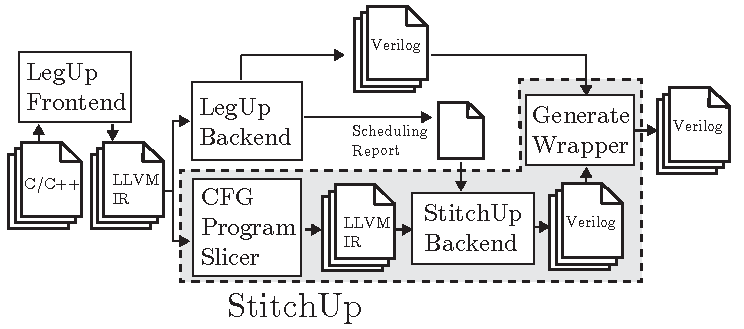
\includegraphics[width=2.5in]{./imgs/tool-flow.pdf}
\caption{Tool Flow Overview diagram}
\label{fig:tool_flow_diagram}
\end{figure}

This section will likely be quite small.

\subsection{Code Analysis Implementation}
What is LLVM? How is the static analysis performed?

\subsection{Code Generation}
What is LegUp? How can this generate StitchUp circuits?


\section{Experiment Setup}
\begin{figure*}[t]
\centering
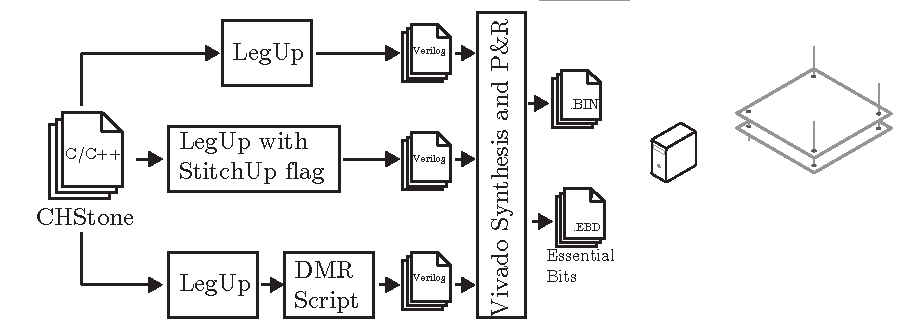
\includegraphics[width=6in]{./imgs/ExperimentFlow.pdf}
\caption{The experiment flow}
\label{fig:ExperimentFlow}
\end{figure*}

To test the error mitigation abilities of StitchUp generated circuits we have adopting the
gold standard of hardware fault injection, where configuration bits on the 
FPGA device are flipped from their original state.
Typical FPGA designs will require a large number of configuration bits often making
full exhaustive testing infeasible, usually resulting in the adoption of random
testing.
However in our case we have developed an experiment
platform allowing us to achieve full exhaustive fault injection in reasonable time,
for example reducing the time to exhaustively test the smallest CHStone circuit dfmul from 4 days
to 8 hours.

We make use of many low cost Xilinx FPGA SoC devices known as
Zedboards all injecting on the same circuit in parallel.
Each Zedboard runs a full Linux OS on its hardened ARM processor, and is arranged into
a cluster managed by a single desktop\footnote{Called The SoC Drawer}.

To flip individual configuration bits a Xilinx Soft Error Mitigation (SEM) IP Core
connected to the FPGA internal configuration port (ICAP) was used --
targeting Xilinx devices was possible due to the latest release of LegUp
(v4.0) which has the ability to generate generic Verilog circuits.
For each experiment the SEM core and the test circuit were instantiated and connected to the
ARM processing system via AXI interconnects.
%Software running under Linux on each ARM core managed each test by first sending an error
%address and injection command to the SEM core, then starting the circuit under test,
%and finally collecting the error (if any) associated with that address.

Figure \ref{fig:ExperimentFlow} shows an overview of the experiment setup.
The top flow generates a standard LegUp circuit with no protection;
the middle uses StitchUp to generate a control-flow structure protected circuit;
and the bottom generates a full DMR protected circuit duplicating the original LegUp
circuit and generating comparison logic on the control FSM state register;

Each different version is then passed through the Xilinx FPGA circuit tool flow to produce
two files: an essential bits file (.EBD), and a configuration binary (.BIN).
The essential bits file is a list of configuration memory bits that have any
influence on our generated circuit and is used to reduce the number of injections
required to fully test our design.\footnote{Essential bits do not contain BRAM data,
since these are considered transient data not essential}
For each experiment the EBD files are divided up into smaller chunks, and each chunk is
processed in parallel on a different Zedboard device.

Software running on the ARM of each Zedboard marshals each test by, injecting a fault,
running the circuit, and storing the result.
The injected fault is then repaired by re-injecting an error into the
same configuration memory location (i.e. flipping the bit back to it's original state).
Some faults may cause the circuit to never terminate, so if no response is seen within three orders
of magnitude of its expected time a, timeout halts its execution.

The results are then analysed and each test outcome is classified into three distinct categories:

\begin{enumerate}
\setlength{\itemsep}{1pt}
\setlength{\parskip}{0pt}
\setlength{\parsep}{0pt}
\item Execution Time Error \textbf{ETE} - This is where the execution of the circuit either took
an incorrect number of cycles to complete or timed out. Errors of these type are
control flow related, since any deviation from the correct execution path will cause
an incorrect number of cycles.
\item Data-Flow Only Errors \textbf{DOE} - These are errors where the circuit has returned an incorrect
data result but has executed in the correct number of cycles, such as error caused
by faults in a non-control structure functional unit.
\item Caught Errors \textbf{CE} - These are errors in the state register that were detected by the protection method, which is
either DMR or StitchUp.
\end{enumerate}

For each test the proportion of ETE, DOE, and CE error results should sum to 100\%.
ETEs are the most critical since they are control related and may runtime guarantees and timeouts;
DOEs are the next critical category since there is an error in data, but no damaging effect on control;
and CEs are the least critical, where the circuit has failed but at least it has been detected.


\section{Experiment Results}
\subsection{Resource Results}
\begin{table*}[t]
\small
\singlespace
\centering
\caption{Resource Usage Results}
\label{tab:resources}
\tabcolsep=0.11cm
\begin{tabular}{@{}|l|l|l|l|l|l|l|l|l|l|l|l|l|@{}}
\toprule
                    & \multicolumn{4}{l|}{\textbf{Original}}                      & \multicolumn{4}{l|}{\textbf{StitchUp}}                      & \multicolumn{4}{l|}{\textbf{DMR}}                           \\ \midrule
\textbf{Benchmarks} & \textit{LUT} & \textit{REG} & \textit{DSP} & \textit{Power} & \textit{LUT} & \textit{REG} & \textit{DSP} & \textit{Power} & \textit{LUT} & \textit{REG} & \textit{DSP} & \textit{Power} \\ \midrule
\textit{aes}        & 47230        & 28152        & 0            &                & 47539        & 28800        & 0            &                &              &              &              &                \\ \midrule
\textit{adpcm}      & 21050        & 16752        & 168          &                & 29599        & 29484        & 178          &                &              &              &              &                \\ \midrule
\textit{blowfish}   &              &              &              &                &              &              &              &                &              &              &              &                \\ \midrule
\textit{dfadd}      & 4639         & 4310         & 0            &                & 5562         & 5095         & 0            &                & 6394         & 5754         & 0            &                \\ \midrule
\textit{dfdiv}      & 12144        & 13157        & 30           &                & 22254        & 23449        & 60           &                & 22811        & 23904        & 60           &                \\ \midrule
\textit{dfmul}      & 3348         & 3912         & 16           &                & 4553         & 4845         & 32           &                & 5105         & 5397         & 32           &                \\ \midrule
\textit{dfsin}      & 21343        & 20347        & 71           &                & 40928        & 38116        & 136          &                &              &              &              &                \\ \midrule
\textit{gsm}        &              &              &              &                &              &              &              &                &              &              &              &                \\ \midrule
\textit{jpeg}       &              &              &              &                &              &              &              &                &              &              &              &                \\ \midrule
\textit{mips}       & 8278         & 6367         & 4            &                & 15639        & 10231        & 8            &                & 14304        & 10351        & 8            &                \\ \midrule
\textit{motion}     &              &              &              &                &              &              &              &                &              &              &              &                \\ \midrule
\textit{sha}        & 9117         & 9287         & 3            &                & 9491         & 10188        & 6            &                & 16788        & 16189        & 6            &                \\ \bottomrule
\end{tabular}
\end{table*}


\begin{figure}[h]
\centering
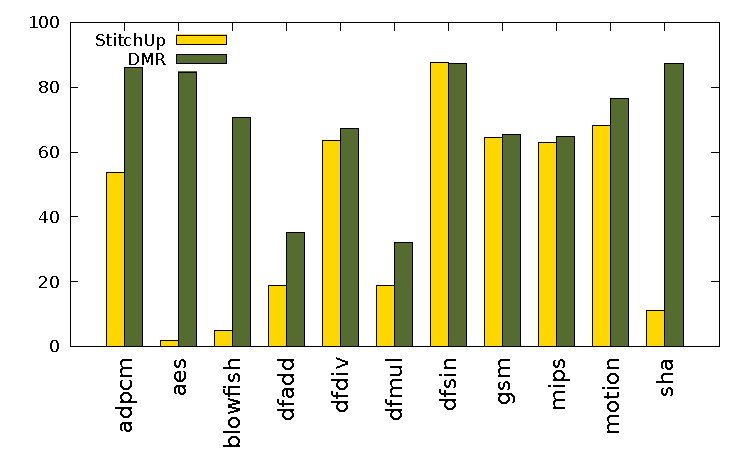
\includegraphics[width=2.5in]{./graphs/chstone_luts_24_09_2015.pdf}
\caption{Luts for the CHStone benchmark}
\label{fig:luts_result}
\end{figure}

\begin{figure}[h]
\centering
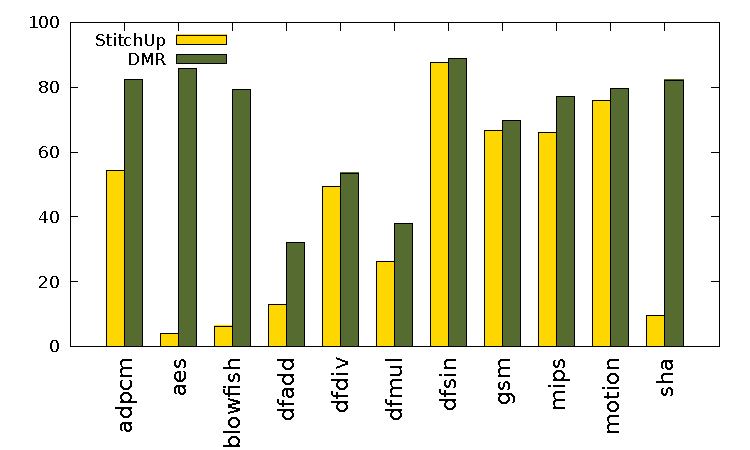
\includegraphics[width=2.5in]{./graphs/chstone_reg_24_09_2015.pdf}
\caption{REGs for the CHStone benchmark}
\label{fig:regs_result}
\end{figure}

\subsection{Power Results}

\begin{figure}[h]
\centering
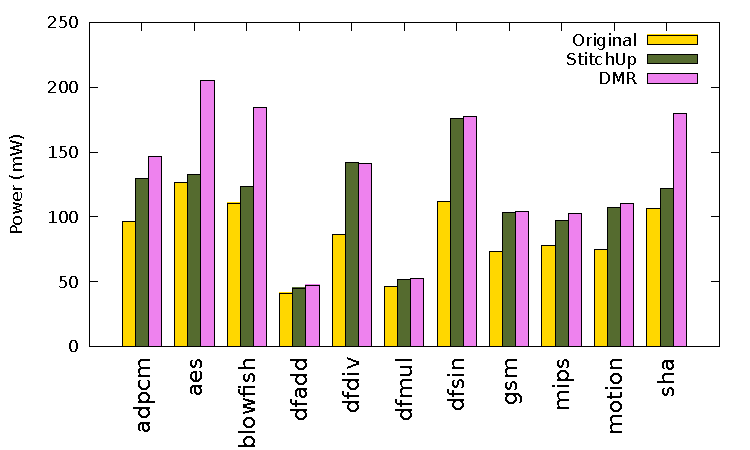
\includegraphics[width=2.5in]{./graphs/chstone_absolute_power_24_09_2015.pdf}
\caption{Power for the CHStone benchmark}
\label{fig:power_result}
\end{figure}

\subsection{Fault Injection Results}


\section{Related Work}
%RELATED WORK SECTION
%Intro to HLS approaches
Early work such as \cite{antola1998high} examined how hardware redundancy 
could be reduced when using HLS to generate DMR circuits.
The authors present a scheduling and alloction algorithm, where the circuit duplication is optimised
so that idle resources are reused instead of instantiating multiple hardware copies.
They manage to successfully reduce the area requirments, while avoiding error aliasing.

%Libary based approaches for Allocation stage of HLS tools
More recent work has instead of using redundancy examined how reliability can be optimised by 
selecting different implementations of components during allocation.
In \cite{tosun2005reliability}
a library of components annotated with area, power, and reliability metrics is used during component selection.    
Initially the set of most reliable components is selected, and then itterative optimisation passes attempt to
meet constraints on the other metrics in a fashion similar to power-aware HLS approaches. 

In \cite{glass2007interactive} this library approach is extended to include the replication of some components 
and an evolutionary algorithm is used to present the results to the user as a design space exploration.
As work in \cite{hara2013cost} extends it to encorporate reliability decisions into scheduling, arguing that
the longer a functional unit is active the more likely it will experience a fault. 

%Application level protection, what can we skip?
The methods discussed so far all propose changes to the underlying HLS algorithms,
none of them  investigate how the input source can be analysed beforehand to extract
critical and non-critical sections of code.
But do such critical and non-critical sections exist?

%HLS methods that exploit the static analysis of input code
Other recent work includes \cite{chen2014reliability} where the vulnerability of variables is analysed and the most vulnerable
variables for a HLS program are protected by assigning them to special registers.
The proposed variable vulnerability analysis takes into account their lifetimes, dependencies, and branch probabilities.
Through analysing the CDFG, error and branch probabilities are used to propagate error likelihood forward to estimate the total
vulnerability for each variable in the design.
A Integer Linear Program solver is then used to minimise the subset of protected registers to cover the maximum number of variables.
They build their results on top of LegUp, and use LLVM to perform the variable vulnerability analysis.
They achieve impressive results, where protecting 20\% of the registers results in more than 60\% soft error mitigation in the best case.
However full fault injection tests are not performed on the generated hardware, and only state-based probabilistic error testing
was performed.\\

%What we are aiming to do differently.


% An example of a floating figure using the graphicx package.
% Note that \label must occur AFTER (or within) \caption.
% For figures, \caption should occur after the \includegraphics.
% Note that IEEEtran v1.7 and later has special internal code that
% is designed to preserve the operation of \label within \caption
% even when the captionsoff option is in effect. However, because
% of issues like this, it may be the safest practice to put all your
% \label just after \caption rather than within \caption{}.
%
% Reminder: the "draftcls" or "draftclsnofoot", not "draft", class
% option should be used if it is desired that the figures are to be
% displayed while in draft mode.
%
%\begin{figure}[!t]
%\centering
%\includegraphics[width=2.5in]{myfigure}
% where an .eps filename suffix will be assumed under latex, 
% and a .pdf suffix will be assumed for pdflatex; or what has been declared
% via \DeclareGraphicsExtensions.
%\caption{Simulation Results}
%\label{fig_sim}
%\end{figure}

% Note that IEEE typically puts floats only at the top, even when this
% results in a large percentage of a column being occupied by floats.


% An example of a double column floating figure using two subfigures.
% (The subfig.sty package must be loaded for this to work.)
% The subfigure \label commands are set within each subfloat command, the
% \label for the overall figure must come after \caption.
% \hfil must be used as a separator to get equal spacing.
% The subfigure.sty package works much the same way, except \subfigure is
% used instead of \subfloat.
%
%\begin{figure*}[!t]
%\centerline{\subfloat[Case I]\includegraphics[width=2.5in]{subfigcase1}%
%\label{fig_first_case}}
%\hfil
%\subfloat[Case II]{\includegraphics[width=2.5in]{subfigcase2}%
%\label{fig_second_case}}}
%\caption{Simulation results}
%\label{fig_sim}
%\end{figure*}
%
% Note that often IEEE papers with subfigures do not employ subfigure
% captions (using the optional argument to \subfloat), but instead will
% reference/describe all of them (a), (b), etc., within the main caption.


% An example of a floating table. Note that, for IEEE style tables, the 
% \caption command should come BEFORE the table. Table text will default to
% \footnotesize as IEEE normally uses this smaller font for tables.
% The \label must come after \caption as always.
%
%\begin{table}[!t]
%% increase table row spacing, adjust to taste
%\renewcommand{\arraystretch}{1.3}
% if using array.sty, it might be a good idea to tweak the value of
% \extrarowheight as needed to properly center the text within the cells
%\caption{An Example of a Table}
%\label{table_example}
%\centering
%% Some packages, such as MDW tools, offer better commands for making tables
%% than the plain LaTeX2e tabular which is used here.
%\begin{tabular}{|c||c|}
%\hline
%One & Two\\
%\hline
%Three & Four\\
%\hline
%\end{tabular}
%\end{table}


% Note that IEEE does not put floats in the very first column - or typically
% anywhere on the first page for that matter. Also, in-text middle ("here")
% positioning is not used. Most IEEE journals/conferences use top floats
% exclusively. Note that, LaTeX2e, unlike IEEE journals/conferences, places
% footnotes above bottom floats. This can be corrected via the \fnbelowfloat
% command of the stfloats package.



\section{Conclusion}
The conclusion goes here.




% conference papers do not normally have an appendix


%\section*{Acknowledgment}


%The authors would like to thank...





% trigger a \newpage just before the given reference
% number - used to balance the columns on the last page
% adjust value as needed - may need to be readjusted if
% the document is modified later
%\IEEEtriggeratref{8}
% The "triggered" command can be changed if desired:
%\IEEEtriggercmd{\enlargethispage{-5in}}

% references section

% can use a bibliography generated by BibTeX as a .bbl file
% BibTeX documentation can be easily obtained at:
% http://www.ctan.org/tex-archive/biblio/bibtex/contrib/doc/
% The IEEEtran BibTeX style support page is at:
% http://www.michaelshell.org/tex/ieeetran/bibtex/
\bibliographystyle{abbrv}
\bibliography{refs.bib}
% argument is your BibTeX string definitions and bibliography database(s)
%\bibliography{IEEEabrv,../bib/paper}
%
% <OR> manually copy in the resultant .bbl file
% set second argument of \begin to the number of references
% (used to reserve space for the reference number labels box)
%\begin{thebibliography}{1}
%
%\bibitem{IEEEhowto:kopka}
%H.~Kopka and P.~W. Daly, \emph{A Guide to \LaTeX}, 3rd~ed.\hskip 1em plus
%  0.5em minus 0.4em\relax Harlow, England: Addison-Wesley, 1999.
%
%\end{thebibliography}




% that's all folks
\end{document}


